\documentclass[12pt]{article}
\usepackage[left=1cm, right=1cm, top=2cm,bottom=1.5cm]{geometry} 

\usepackage[parfill]{parskip}
\usepackage[utf8]{inputenc}
\usepackage[T2A]{fontenc}
\usepackage[russian]{babel}
\usepackage{enumitem}
\usepackage[normalem]{ulem}
\usepackage{amsfonts, amsmath, amsthm, amssymb, mathtools}

\usepackage{accents}
\usepackage{fancyhdr}
\pagestyle{fancy}
\renewcommand{\headrulewidth}{1.5pt}
\renewcommand{\footrulewidth}{1pt}

\usepackage{graphicx}
\usepackage[figurename=Рис.]{caption}
\usepackage{subcaption}
\usepackage{float}

%%Наименование папки откуда забирать изображения
\graphicspath{ {./images/} }

%%Изменение формата для ввода доказательства
\renewcommand{\proofname}{$\square$  \nopunct}
\renewcommand\qedsymbol{$\blacksquare$}

\addto\captionsrussian{%
	\renewcommand{\proofname}{$\square$ \nopunct}%
}
%% Римские цифры
\newcommand{\RN}[1]{%
	\textup{\uppercase\expandafter{\romannumeral#1}}%
}

%% Для удобства записи
\newcommand{\MR}{\mathbb{R}}
\newcommand{\MQ}{\mathbb{Q}}
\newcommand{\MI}{\mathrm{I}}
\newcommand{\MJ}{\mathrm{J}}
\newcommand{\MH}{\mathrm{H}}
\newcommand{\MT}{\mathrm{T}}
\newcommand{\MU}{\mathcal{U}}
\newcommand{\MV}{\mathcal{V}}
\newcommand{\VN}{\varnothing}
\newcommand{\VE}{\varepsilon}

\theoremstyle{definition}
\newtheorem{defn}{Опр:}
\newtheorem{rem}{Rm:}
\newtheorem{prop}{Утв.}
\newtheorem{exrc}{Упр.}
\newtheorem{lemma}{Лемма}
\newtheorem{theorem}{Теорема}
\newtheorem{corollary}{Следствие}

\newenvironment{cusdefn}[1]
{\renewcommand\thedefn{#1}\defn}
{\enddefn}

\DeclareRobustCommand{\divby}{%
	\mathrel{\text{\vbox{\baselineskip.65ex\lineskiplimit0pt\hbox{.}\hbox{.}\hbox{.}}}}%
}
%Коротки минус
\DeclareMathSymbol{\SMN}{\mathbin}{AMSa}{"39}

\newcommand{\smallerrel}[1]{\mathrel{\mathpalette\smallerrelaux{#1}}}
\newcommand{\smallerrelaux}[2]{\raisebox{.1ex}{\scalebox{.75}{$#1#2$}}}

\newcommand{\smallin}{\smallerrel{\in}}
\newcommand{\smallnotin}{\smallerrel{\notin}}

\newcommand*{\medcap}{\mathbin{\scalebox{1.25}{\ensuremath{\cap}}}}%
\newcommand*{\medcup}{\mathbin{\scalebox{1.25}{\ensuremath{\cup}}}}%

%Подпись символов снизу
\newcommand{\ubar}[1]{\underaccent{\bar}{#1}}

\begin{document}
\lhead{Математический анализ - I}
\chead{Шапошников С.В.}
\rhead{Лекция - 26}

\section*{Формула Тейлора. Ряды Тейлора}

Формула Тейлора с остаточным членом:
$$f(x) = \sum\limits_{k = 0}^{n}\dfrac{f^{(k)}(a)(x-a)^k}{k!} + r_n(x,a)$$

\begin{defn}
	Если функция $f$ бесконечное число раз дифференцируема в окрестности точки $a$, то ряд $$\sum\limits_{k = 0}^{\infty}\dfrac{f^{(k)}(a)(x-a)^k}{k!}$$ 
	называется \uwave{рядом Тейлора в точке $a$ функции $f$}.
\end{defn}

\textbf{Пример Коши}: $f(x) = \begin{cases} 0, & x\leq 0\\ e^{-\frac{1}{x}}, & x > 0 \end{cases}$

$f$ бесконечное число раз дифференцируема (в том числе в 0) и $f^{(n)}(0) = 0$.
\begin{figure}[H]
	\centering
	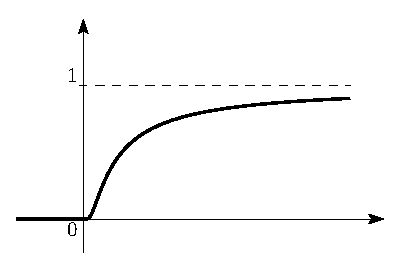
\includegraphics[width=0.35\textwidth]{26_1.eps}
	\caption{Пример Коши.}
	\label{26_1}
\end{figure}
Посчитаем её производную: 
$$f^\prime(0) = \lim\limits_{x\to 0+}\dfrac{f(x)- f(0)}{x-0} = \lim\limits_{x \to 0+}\dfrac{e^{-\frac{1}{x}}}{x} \underset{t =\frac{1}{x}}{=} \lim\limits_{x \to +\infty}te^{-t} = \lim\limits_{x \to +\infty}\frac{t}{e^{t}} = \lim\limits_{x \to +\infty}\frac{1}{e^{t}} = 0$$

Ряд Тейлора для этой функции равен $\displaystyle \sum\limits_{k = 0}^{\infty}\dfrac{0{\cdot}x^k}{k!}\equiv 0$, но она ни в какой окрестности нуля не является тождественно нулевой. Таким образом, ни на каком интервале вокруг точки $0$ эта сумма не сходится к нашей функции.

\begin{theorem}\textbf{(Борель)}:
	Для всякой числовой последовательности $\{c_n\}$ существует бесконечно дифференцируемая в окрестности $x=0$ функция $f\colon f^{(n)}(0) = c_n$.
\end{theorem}

\textbf{Пример}: $c_n = (n!)^2 \Rightarrow \displaystyle \sum\limits_{k = 0}^{\infty}k!x^k$ - ряд Тейлора, сходится только в одной точке: $x = 0$.

\begin{theorem}
	Пусть $f$ бесконечно дифференцируема на интервале $(a-r,a+r)$ и \\
	$\sup\limits_{x \in (a-r,a+r)}|f^{(n)}(x)| \leq C{\cdot}q^n{\cdot}n!$, где $C >0, \, 0 < q < \frac{1}{r}$. Тогда $$\displaystyle \sum\limits_{k = 0}^{\infty} \dfrac{f^{(k)}(a)(x-a)^k}{k!}$$ сходится равномерно к $f(x)$ для всякого $x \in (a - r, a + r)$ 
\end{theorem}
\begin{proof}
	Используем остаточный член в форме Лагранжа:
	$$\bigg|f(x) - \sum\limits_{k = 0}^{n} \dfrac{f^{(k)}(a)(x-a)^k}{k!} \bigg| = \bigg|\dfrac{f^{(n+1)}(c)(x-a)^{n+1}}{(n+1)!} \bigg|, \, c \in (a,x) \vee c \in (x,a)$$
	Так как $|x - a| < r, \, c \in (a,x) \vee c \in (x,a) \Rightarrow c \in (a-r, a+r) \Rightarrow$
	$$\bigg|\dfrac{f^{(n+1)}(c)(x-a)^{n+1}}{(n+1)!} \bigg| \leq \dfrac{Cq^{n+1}{\cdot}(n+1)!{\cdot}r^{n+1}}{(n+1)!} = C(qr)^{n+1}, \, 0 < q < \frac{1}{r} \Rightarrow (qr) < 1 \Rightarrow (qr)^{n+1} \xrightarrow[n \to \infty]{} 0$$
\end{proof}

\textbf{Пример}: $e^x, \, a = 0 \Rightarrow |e^x| \leq Cq^n n!,\, 0 < q < \frac{1}{r} $. Но на любом интервале $e^x$ - ограниченна, $r$ - любое, а $\forall q, \, q^n n! \to \infty \Rightarrow$ после выбора $C$ данная оценка будет верна на каждом интервале. 

\begin{defn}
	Функция $f$ называется \uwave{аналитической} в окрестности $\MU(a)$ точки $a$, если она бесконечно дифференцируема и её ряд Тейлора сходится к $f$ на окрестности $\MU(a)$.
\end{defn}

\textbf{Пример}: $\dfrac{1}{1+x^2}$ - бесконечно дифференцируемая функция. Напишем её ряд Тейлора в $0$: 
$$\dfrac{1}{1+x^2} = \displaystyle \sum\limits_{k=0}^{\infty}(-1)^k x^{2k}$$
Ряд сходится при $x \in (-1,1)$, но при этом значения функции в точках $|x| \geq 1$ определены. По оси вещественных чисел $x$ нет проблем, но на комплексной плоскости есть две плохие точки $i,-i$.

\begin{rem} \textbf{(Метод неопределенных коэффициентов)}
	Пусть $f(x) = c_0 + c_1(x-a) + \dotsc + c_n(x-a)^n + \underset{x \to a}{\bar{o}((x-a)^n)} \Rightarrow$ коэффициенты $c_k$ определены однозначно. $c_0 = \lim\limits_{x \to a} f(x), \, c_1 = \lim\limits_{x \to a} \dfrac{f(x) - c_0}{x-a}, \dotsc \Rightarrow$ так как предел определен единственным образом, то на каждом шаге предыдущие коэффициенты найдены, поэтому нет никакой неопределенности в выборе коэффициентов.
\end{rem}

\textbf{Пример}: $(\tg{x})^\prime = 1 + \tg^2{x}$. Найдем разложение $\tg{x}$: понимаем, что эта функция нечетная $\Rightarrow$ разложение не будет содержать коэффициенты четной степени, поскольку все четные производные будут равны $0 \Rightarrow \tg{x} = c_1x + c_3x^3 + c_5x^5 + \dotsc$. Предположим мы знаем, что эту сумму можно почленно дифференцировать $\Rightarrow$
$$c_1 + 3c_3x^2 + 5c_5x^4 + \dotsc = 1 + (c_1x + c_3x^3 + c_5x^5 + \dotsc)^2\Rightarrow c_1 = 1, \, 3c_3 = c_1^2 \Rightarrow c_3 = \frac{1}{3}, \, \dotsc$$  

\newpage
\section*{Свойства производной. Непрерывность $f^\prime$}

Пусть $f$ дифференцируема всюду на $\MR \Leftrightarrow \exists \, f^\prime(x) = \lim\limits_{h \to 0} \dfrac{f(x+h) - f(x)}{h}$. По определению Гейне, если такой предел есть, его можно брать по любой последовательности, подходящей к $x$. 

Рассмотрим $f_n(x) = n(f(x + \frac{1}{n}) - f(x)) \Rightarrow f_n(x)$ поточечно сходится к $f^\prime$. Функция всюду дифференцируема $\Rightarrow$ она всюду непрерывна $\Rightarrow f_n$ - непрерывные функции. Поточечный предел непрерывных функций имеет всюду плотное множество точек непрерывности $\Rightarrow$ у $f^\prime$ всюду плотное множество точек непрерывности. 

Тогда $f^\prime$ не может оказаться, например, функцией Дирихле или функцией у которой только одна точка непрерывности, но при этом $f^\prime$ может иметь разрыв.

\textbf{Пример}: $f(x) = \begin{cases} x^2\sin{\frac{1}{x}}, & x \neq 0\\  0, &  x = 0
\end{cases}$. 

Если $x \neq 0 \Rightarrow f^\prime(x) = 2x\sin{\frac{1}{x}} - \cos{\frac{1}{x}}$. Если $x = 0 \Rightarrow f^\prime(0) = \lim\limits_{x \to 0}\dfrac{f(x) - 0}{x - 0} = \lim\limits_{x \to 0}\dfrac{x^2 \sin{\frac{1}{x}}}{x} = 0$. 

Функция всюду дифференцируема, но $f^\prime$ имеет разрыв $\RN{2}$-го рода в точке $x = 0$. 

Возможны ли устранимые разрывы или разрывы \RN{1}-го рода? Рассмотрим следующую теорему.

\begin{theorem}\textbf{(Дарбу)}
	Пусть $f$ дифференцируема в каждой точке отрезка $[a,b]$ и $f^\prime(a){\cdot}f^\prime(b) < 0$. Тогда $\exists \, c \in [a,b] \colon f^\prime(c) = 0$.
\end{theorem}
\begin{proof}
	Пусть $f^\prime(a) < 0 \wedge f^\prime(b)>0 \Rightarrow 0 > f^\prime(a) = \lim\limits_{x \to a}\dfrac{f(x) - f(a)}{x - a} \Rightarrow$ в окрестности точки $a$ данное отношение будет меньше $0 \Rightarrow \exists \, \delta > 0 \colon \forall x \in (a, a + \delta), \, \dfrac{f(x) - f(a)}{x-a} < 0 \wedge x > a \Rightarrow f(x) < f(a)$.
	\begin{figure}[H]
		\centering
		\includegraphics[width=0.4\textwidth]{26_2.eps}
		\caption{Доказательство теоремы Дарбу.}
		\label{26_2}
	\end{figure}
	Поскольку $0 < f^\prime(b) = \lim\limits_{x \to b}\dfrac{f(x) - f(b)}{x - b} \Rightarrow \exists \, \tilde{\delta} > 0 \colon \forall x \in (b -\tilde{\delta}, b), \, \dfrac{f(x) - f(b)}{x-b} > 0 \wedge x < b \Rightarrow f(x) < f(b)$.
	
	Поскольку функция дифференцируема на отрезке $\Rightarrow$ она непрерывна на нем и принимает свое наименьшее и наибольшее значения. Таким образом, $\min\limits_{[a,b]}f \neq f(a) \wedge \min\limits_{[a,b]}f \neq f(b) \Rightarrow$  минимум достигается в некоторой точке $c$ внутри отрезка и по теореме Ферма $f^\prime(c) = 0$.
\end{proof}

\begin{corollary}
	Если $f$ дифференцируема в каждой точке отрезка $[a,b]$ и $A = f^\prime(a), \, B = f^\prime(b)$, то \\
	$\forall C$ между $A$ и $B$ найдется $c \in [a,b] \colon f^\prime(c) = C$.
\end{corollary}
 
\begin{proof}
	Рассмотрим функцию $g(x) = f(x) - Cx \Rightarrow$ проверяется сразу, что $g^\prime(a)g^\prime(b) = (A-C)(B-C) \leq 0$.
	
	Если $g^\prime(a)g^\prime(b) = 0 \Rightarrow$ производная совпала со значением или в точке $a$, или в точке $b$.
	
	Если $g^\prime(a)g^\prime(b) < 0 \Rightarrow$ по теореме Дарбу $\exists \, c \in [a,b] \colon g^\prime(c) = 0 \Rightarrow f^\prime(c) - C = 0 \Rightarrow f^\prime(c) = C$.
\end{proof}

Таким образом, производная обладает свойством промежуточного значения $\Rightarrow$ не может быть разрывов ни \RN{1}-го рода, ни устранимых, а возможны лишь разрывы \RN{2}-го рода

\section*{Правило Лейбница для производных высокого порядка}
\begin{theorem}
	Пусть $f$ и $g$ $n$-раз дифференцируемы в точке $a$. Тогда $f{\cdot}g$  $n$-раз дифференцируема и верно равенство:
	$$(fg)^{(n)}(a) = \sum\limits_{k = 0}^{n}C_n^k{\cdot}f^{(k)}(a){\cdot}g^{(n-k)}(a)$$
\end{theorem}
\begin{proof} Докажем по индукции:\\
	\uline{\textbf{База}}: обычное правило Лейбница $(fg)^\prime = f^\prime g + fg^\prime = C_1^0 f^{(0)}g^{(1)} + C_1^1 f^{(1)}g^{(0)}$. Рассмотрим вторую производную, как производную от прозводной первого порядка: $(fg)^{\prime\prime} = (f^\prime g + fg^\prime)^\prime = f^{\prime\prime}g + 2f^\prime g^\prime + g^{\prime\prime}f$.
	
	\uline{\textbf{Шаг}}: пусть доказано для $n$, докажем для $n +1$:
	$$(fg)^{(n+1)} = ((fg)^{(n)})^\prime =  \sum\limits_{k=0}^{n}C_n^k \big(f^{(k+1)}g^{(n - k)} + f^{(k)}g^{(n + 1 - k)}\big) = $$ 
	$$= fg^{(n+1)} + f^{(n+1)}g + \sum\limits_{m=1}^{n} \big(C_n^{m-1} + C_n^m \big) f^{(m)}g^{(n+1-m)}  = \sum\limits_{m=0}^{n + 1} C_{n+1}^m f^{(m)}g^{(n + 1 - m)}$$
\end{proof}

\textbf{Пример}: $(xe^x)^{(n)} = \displaystyle \sum\limits_{k = 0}^{n}C_n^k{\cdot}(x)^{(k)}{\cdot}(e^x)^{(n-k)} = C_n^0{\cdot}xe^x + C_n^1{\cdot}e^x = xe^x + ne^x$.

\newpage
\section*{Исследование функций}
\begin{defn}
	Точка $a$ называется \uwave{точкой локального (внутреннего) минимума} (\uwave{максимума)} функции $f$, если $f$ определена в окрестности $\MU(a)$ точки $a$ и $\forall x \in \MU(a), \, f(x) \geq f(a) \; (f(x) \leq f(a))$. 
\end{defn}

\begin{defn}
	Точка $a$ называется \uwave{точкой строгого локального (внутреннего) минимума} (\uwave{максимума)}  функции $f$, если $f$ определена в окрестности $\MU(a)$ точки $a$ и $\forall x \in \MU^\prime(a), \, f(x) > f(a) \; (f(x) < f(a))$. 
\end{defn}

\begin{defn}
	Точки локального минимума или максимума называются \uwave{точками локального (внутреннего) экстремума $f$}.
\end{defn}

\begin{figure}[H]
	\centering
	\includegraphics[width=0.25\textwidth]{26_3.eps}
	\caption{Не внутренние максимумы и минимумы.}
	\label{26_3}
\end{figure}

\begin{theorem}\textbf{(Ферма)} \textbf{Необходимое условия локального экстремума}:
	Если функция $f$ дифференцируема в точке $a$ и точка $a$ это точка внутреннего локального экстремума, то $f^\prime(a) = 0$.
\end{theorem}

\end{document}